\section{Eliminar Doctor}

Un paciente podrá eliminar un doctor en caso de que el doctor ya no sea responsable de ningún tratamiento.

\subsubsection{Procedimiento}
\begin{enumerate}
	
	\item Selecciona el doctor que deseas eliminar en la pantalla \textbf{Doctores}.
	
	\begin{figure}[!htbp]			
		\hypertarget{fig:Doctores2}{\hspace{1pt}}
		\begin{center}
			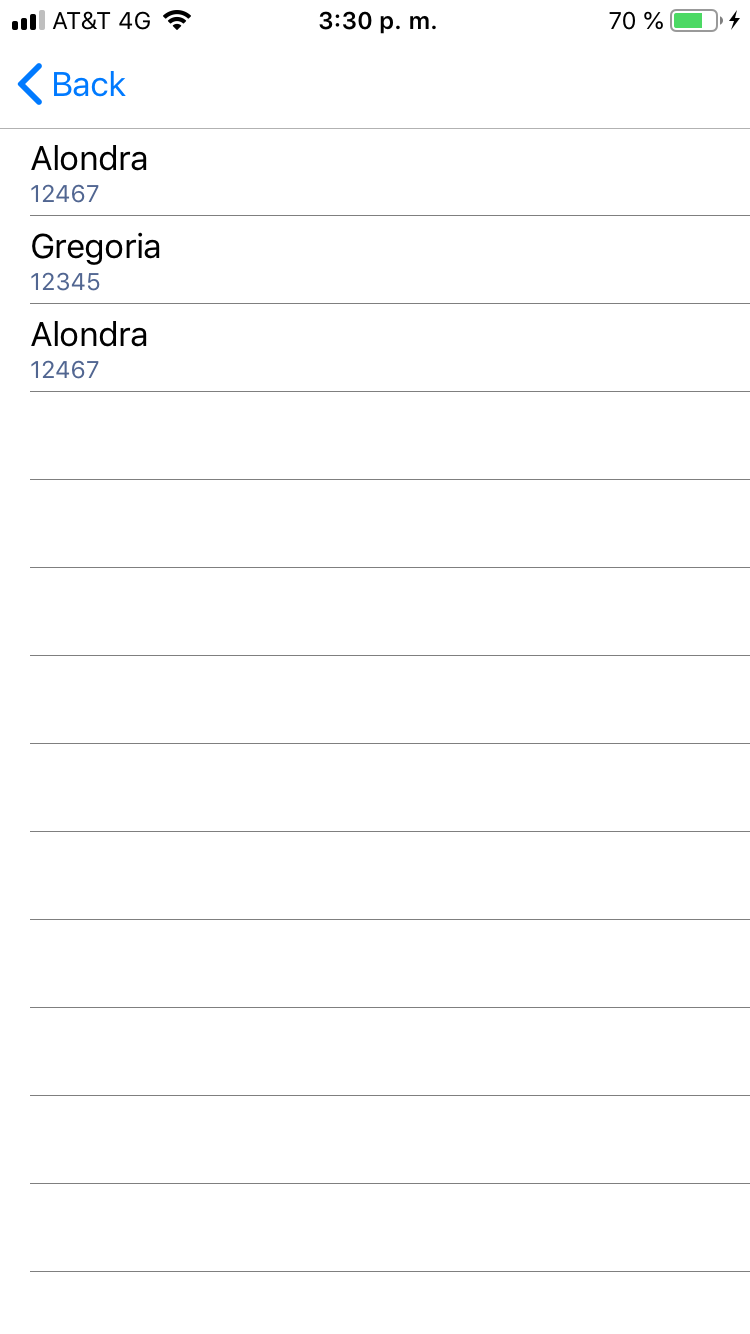
\includegraphics[height=0.4\textheight]{Paciente/EliminarDoctor/images/Doctores}
			\caption{Doctores}
			\label{fig:Doctores2}
		\end{center}
	\end{figure}

	\item Se mostrará la pantalla \textbf{Información del Doctor}.
	\newpage
	\begin{figure}[!htbp]			
		\hypertarget{fig:InfoDoctor}{\hspace{1pt}}
		\begin{center}
			
\includegraphics[height=0.4\textheight]{Paciente/EliminarDoctor/images/InfoDoctor}
			\caption{Información del Doctor}
			\label{fig:InfoDoctor}
		\end{center}
	\end{figure}

	\item Da clic en el botón \textbf{Eliminar Doctor}.
	
\end{enumerate}

